
\RequirePackage{fix-cm}
%
%\documentclass{svjour3}                     % onecolumn (standard format)
%\documentclass[smallcondensed]{svjour3}     % onecolumn (ditto)
%\documentclass[smallextended]{svjour3}       % onecolumn (second format)
\documentclass[twocolumn]{svjour3}          % twocolumn
\smartqed  % flush right qed marks, e.g. at end of proof
\usepackage{graphicx}
\usepackage{amsfonts,amssymb,amsmath,
            amssymb,amsopn,amsxtra,amstext,amsbsy}
\usepackage{epsfig}
\usepackage[makeroom]{cancel}
\usepackage{array,arydshln}
\usepackage{array}
\usepackage{url}
%\usepackage{tikz}
\usepackage[utf8x]{inputenc}
\usepackage{fancyhdr}
\usepackage{hyperref,wasysym}
\usepackage{color}
\usepackage{enumerate}
\usepackage{algorithm}
\usepackage{algorithmic}
\renewcommand{\algorithmicrequire}{\textbf{Input:}}
\renewcommand{\algorithmicensure}{\textbf{Output:}}
\usepackage{multirow}
%\usepackage[spanish]{babel}

\usepackage{xcolor}
\usepackage{hyperref}
\usepackage{pmat}


\journalname{Applied Intelligence}


\begin{document}

\title{High frequency intraday forex rates forecasting using an online cointegration approach}
%\subtitle{Do you have a subtitle?\\ If so, write it here}

%\titlerunning{Short form of title}        % if too long for running head

\author{Paola Arce \and Werner Kristjanpoller \and Luis Salinas }

%\authorrunning{Short form of author list} % if too long for running head

\institute{P. Arce  \at
              Departamento de Inform\'atica, Universidad T\'ecnica Federico Santa
              Mar\'ia\\
              Tel.: +56-32-2654000\\
              %Fax: +123-45-678910\\
              \email{paola.arce@usm.cl}           %  \\
%             \emph{Present address:} of F. Author  %  if needed
           \and
           W. Kristjanpoller \at
              Departamento de Industrias, Universidad T\'ecnica Federico Santa
              Mar\'ia\\
              %Fax: +123-45-678910\\
              \email{werner.kristjanpoller@usm.cl}             \\
           \and
           L. Salinas \at
              Departamento de Inform\'atica, Universidad T\'ecnica Federico Santa
              Mar\'ia\\
              Centro Científico Tecnológico de Valparaíso (CCTVal) \\
              \email{luis.salinas@usm.cl}           %  \\
}

\date{Received: date / Accepted: date}
% The correct dates will be entered by the editor


\maketitle

\begin{abstract}

This research examines the cointegration relation between three mayor currency pairs (MCP) of the foreign exchange markets:  EURUSD, GBPUSD, USDCHF. Specifically, we used a modified version of the Vector error correction model (VECM) which parameters are updated online using a limited amount of historical data.
VECM parameters are commonly obtained using the
ordinary least squares (OLS) method. Our proposal is to solve VECM using Ridge regression (RR) and the Aggregating algorithm for regression (AAR) which could lead to a better generalisation capability rather than OLS. Both approaches together with OLS are compared against an optimal offline algorithm which is able to see the sequences in advance.
Our experiments were carried out using 10-seconds frequency Forex data and shows that RR and AAR approaches improve cumulative loss of OLS approach with respect to the optimal offline algorithm.


\keywords{VECM \and Cointegration \and Forex \and High frequency data \and Online algorithm}

\end{abstract}

\section{Introduction}
\label{sec:introduction}

The relationships between financial time series are commonly studied. In particular, in some of them
it is possible to detect long-run relationships through to a cointegration analysis. Two or more non-stationary time series are said to be cointegrated if there exists a linear combination of them which is stationary.

The vector error correction model (VECM) introduces the long-run relationship among a set of cointegrated variables
as an error correction term. VECM is a special case of the vector autoregressive
model (VAR) model. VAR model expresses future values as a linear combination of
variables past values.  However, VAR model cannot be used with non-stationary
variables, which is a common feature of financial assets. VECM is a linear model
but in terms of variable differences. If cointegration exists, variable
differences are stationary and they introduce an error correction term which
adjusts coefficients to bring the variables back to equilibrium. In finance,
many economic time series turns out to be stationary, when they are differentiated once (see section \ref{sec:coint} for more details). Additionally, cointegration restrictions applied on the model often improves forecasting~\cite{duy1998}. This is the reason why VECM has been widely adopted.

VECM parameters are obtained using ordinary least squares
(OLS) method \cite{golub1980}. OLS has two main problems: it is sensitive to errors on input data
and also involves many calculations. The former problem is commonly solved using
Ridge Regression (RR) \cite{hoerl1970} which introduces a regularisation
parameter that leads to an unbiased estimation with better generalisation
capability. The second problem of computational complexity depends on the number
of past values and observations considered.  Recently, online learning
algorithms have been proposed to solve problems with large data sets because of
their simplicity and their ability to update the model when new data is
available. We use an online version of the linear ridge regression and also a modification introduced by 
Vovk \cite{vovk2001} called the Aggregating algorithm regression (AAR).
Our proposal is an online formulation of the VECM called Online VECM (OVECM)
based on the consideration of only a sliding window of the historical data at every step.  OVECM parameters are obtained via OLS, RR or AAR. In order to measure performance, a competitive analysis is done which compares the proposal cumulative loss against the optimal offline algorithm. 

In finance, little academic research has been done using high-frequency Forex
rates \cite{Bekiros2015}. Our proposal is tested using
three mayor currency pairs (MCP) from the foreign exchange market:  Euro (EUR) to United States Dollar (USD) (EURUSD), British Pound (GBP) to
USD (GBPUSD) and USD to Swiss Franc (CHF) (USDCHF). We used samples with a frequency of 10 seconds.

This paper is organised as follows: section~\ref{sec:background} presents concepts of integration and cointegration, the VECM model and an online learning introduction, the OVECM algorithm is presented in section~\ref{sec:methodology}.
In section~\ref{sec:results} we describe the experiments carried out and their results. This section also includes a
description of the test data.  Section~\ref{sec:conclusions} contains the
conclusions and a discussion of future research.


\section{Background}
\label{sec:background}
\subsection{Integration and Cointegration}\label{sec:coint}\  
Following Johansen \cite{johansen1995} we shall say that a stochastic process
$Y_t$ which satisfies $Y_t-E(Y_t) = \sum_{i=0}^\infty C_i\,\varepsilon_{t-i}$ is
called $I(0)$, and then we shall write $Y_t\sim I(0)$, whenever
$\sum_{i=0}^\infty C_i \neq 0$ and $\sum_{i=0}^\infty C_i\,z^i$ converges for
$z\in\mathbb{C}$ with $|z|<1$.  It is understood that the condition
$\varepsilon_t\sim iid(0,\sigma^2)$ holds.

A (vector) time series $\mathbf{y}_t$ is said to be {\em integrated of order\/}
$d$, and then we shall write $\mathbf{y}_t\sim I(d)$, whenever after $d$ times
(discrete) differentiation an stationary process is obtained~\cite{banerjee1993};
more precisely, whenever
$(1-L)^d\,\mathbf{y}_t\sim\text{I(0)}$, where $L$ is the usual lag operator:
$(1-L)\,\mathbf{y}_t = \Delta\mathbf{y}_t = \mathbf{y}_t-\mathbf{y}_{t-1}$ for
all $t$.  

Note that this definition includes the scalar case as time series of
vectors of dimension 1; in this scalar case we will write the time series in
nonbold format.

Let $\mathbf{y}_t^\nu$, $\nu=1,\dots,p$, be a set of $p$ vector time series of
order $I(1)$.  They are said to be {\em cointegrated\/} if a vector
$\beta=[\beta(1),\dots,\beta(p)]^\top \in \mathbb{R}^p$ exists, such that the
time series,
\begin{equation}
\mathbf{Z}_t:= 
\sum_{\nu=1}^p \beta(\nu)\,\mathbf{y}_t^\nu\,\sim\,\text{I(0)}\,.
\end{equation}
In other words, a set of $I(1)$ time series is said to be cointegrated if a
linear combination of them exists, which is I(0).


\subsection{Vector Error Correction Model}\label{sec:varvec}

VECM is a special case of VAR model and both describe the joint behaviour
of a set of variables.

The VAR($p$) model is a general framework describing the behaviour of a
set of $l$ endogenous variables as a linear combination of their last $p$
values, where $l,p\in\mathbb{N}$. 
In our case, each one of these $l$ variables is a scalar time series
$y_{\lambda,t}$, $\lambda=1,\dots,l$, and we represent them all together
at time $t$ by the the vector time series:
\begin{equation}
\label{eq:variables}
\mathbf{y}_t = 
\begin{bmatrix} y_{1,t} & y_{2,t} & \dots & y_{l,t} \end{bmatrix}^\top.
\end{equation}
\noindent
Notice that the vectors $\mathbf{y}_t$ are assumed to be $l$-dimensional.

The VAR($p$) model describes the behaviour of a dependent variable in terms of
its own lagged values and the lags of the others variables in the system. The
model with $p$ lags is formulated as the system of $N$:
\begin{align}
\label{eq:var}
\mathbf{y}_t 
= \boldsymbol{\Phi}_1 \mathbf{y}_{t-1} +
  \boldsymbol{\Phi}_2 \mathbf{y}_{t-2} + \dots +
  \boldsymbol{\Phi}_p\mathbf{y}_{t-p} +
  \mathbf{c} + \boldsymbol{\epsilon}_t \nonumber \\
t=p+1,\dots,N,
\end{align}
\noindent where 
$\boldsymbol{\Phi}_1, \boldsymbol{\Phi}_2,\dots,\boldsymbol{\Phi}_p$
are $l\times l$-matrices of real coefficients,
$\boldsymbol{\epsilon}_{p+1},
 \boldsymbol{\epsilon}_{p+2}, \dots, \boldsymbol{\epsilon}_N$ 
are error terms, $\mathbf{c}$ is a constant vector and $N$ is the total
number of samples.

Notice that, regarding our notation of section (\ref{sec:coint}),
we have here 
$\mathbf{y}_t^0 = \mathbf{y}_t$,
$\mathbf{y}_t^\nu = \mathbf{y}_{t-\nu}$ and
the $\lambda$-th component of the vector time series $\mathbf{y}_t^\nu$
is the scalar time series $y_{\lambda,t}^\nu$, where $\nu=1,\dots,p$ and
$\lambda=1,\dots,l$.

VECM is a special form of a VAR model for I(1) variables that are also
cointegrated~\cite{johansen1991,banerjee1993}.

It is obtained re-writing equation (\ref{eq:var}) in terms of the new
variable $\Delta\mathbf{y}_t=\mathbf{y}_t-\mathbf{y}_{t-1}$.
The VECM model, expressed in terms those differences, takes the form:
\begin{equation}\label{eq:vec}
\Delta \mathbf{y}_t 
= \boldsymbol{\Omega}\,\mathbf{y}_{t-1}
  + \sum_{i=1}^{p-1} \boldsymbol{\Phi}_i^*\,\Delta\mathbf{y}_{t-i}
  + \mathbf{c} + \boldsymbol{\epsilon}_t\,,
\end{equation}
\noindent
where the coefficients matrices $\boldsymbol{\Phi}_i^*$ and 
$\boldsymbol{\Omega}$, expressed in terms of the matrices
$\boldsymbol{\Phi}_i$ of (\ref{eq:var}), are:
\begin{align*}
\boldsymbol{\Phi}_i^* 
&:= -\sum_{j=i+1}^{p}\boldsymbol{\Phi}_j\,, \\
\boldsymbol{\Omega}
&:= -\left( \mathbb{I} - \boldsymbol{\Phi}_1 - \dots 
    - \boldsymbol{\phi}_p \right)\,. 
\end{align*}
The following well known properties of the matrix $\boldsymbol{\Omega}$
\cite{johansen1995} will be useful in the sequel:
\begin{itemize}
\item
If $\boldsymbol{\Omega} = \mathbf{0}$, there is no cointegration.
\item 
If $rank(\boldsymbol{\Omega})=l$, i.e., if $\boldsymbol{\Omega}$ has
full rank, then the time series are not I(1) but stationary.
\item
If $rank(\boldsymbol{\Omega})=r$, $0<r<l$, then there is cointegration
and the matrix $\boldsymbol{\Omega}$ can be expressed as
$\boldsymbol{\Omega}=\boldsymbol{\alpha\beta}^\top$, where $\boldsymbol{\alpha}$
and $\boldsymbol{\beta}$ are
$l\times r$ matrices and
$\text{rank}(\boldsymbol{\alpha})=\text{rank}(\boldsymbol{\beta})=r$.
\item
The columns of $\boldsymbol{\beta}$ contains the cointegration vectors and the rows of
$\boldsymbol{\alpha}$ correspond with the adjusted vectors. 
$\boldsymbol{\beta}$ is obtained by Johansen procedure~\cite{johansen1988},
whereas $\boldsymbol{\alpha}$ has to be determined as a variable in the VECM.
\end{itemize}
It is worth noticing that the factorization of the matrix
$\boldsymbol\Omega$ is not unique, since for any $r \times r$
non-singular matrix $\mathbf{H}$, $\boldsymbol{\alpha}^*:=\boldsymbol{\alpha}\mathbf{H}$,
and $\boldsymbol{\beta}^*=\boldsymbol{\beta}(\mathbf{H}^{-1})^\top$ we have
$\boldsymbol{\alpha\beta}^\top=\boldsymbol{\alpha}^*(\boldsymbol{\beta}^*)^\top$.
If cointegration exists, then equation (\ref{eq:vec}) can be written
as follows:
\begin{equation}\label{eq:vecfull}
\Delta\mathbf{y}_t 
= \boldsymbol{\alpha\beta}^\top\mathbf{y}_{t-1} 
  + \sum_{i=1}^{p-1}\boldsymbol{\Phi}_i^*\,\Delta\mathbf{y}_{t-i}
  + \mathbf{c} + \boldsymbol{\epsilon}_t\,,
\end{equation}
\noindent
which is a VAR model but for time series differences ~\cite{hansen1999}.


Transposing each equation of the system (\ref{eq:vecfull}) we can write
the VECM($p$) model in block-matrix form as:
\begin{equation}\label{eq:vareq}
\mathbf{Y} = 
\mathbf{A} \mathbf{X} + 
\mathbf{E} \, , 
\end{equation}
%
\noindent where $\mathbf{Y}$ dimension is $((N-p)\times l)$, $\mathbf{A}$
dimension is $((N-p)\times(r+(p-1)l +1))$, $\mathbf{X}$ dimension is $((r+(p-1)l
+1)\times l)$ and $\mathbf{E}$ dimension is $((N-p)\times l)$:
%
\begin{alignat}{3}
\mathbf{Y}
&= \begin{bmatrix}
   \Delta\mathbf{y}_{p+1}^\top \\
   \Delta\mathbf{y}_{p+2}^\top \\
   \vdots \\
   \Delta\mathbf{y}_N^\top
   \end{bmatrix}
&\quad
\mathbf{X}
&= \begin{bmatrix}
   \boldsymbol{\alpha}^\top \\
   \boldsymbol{\Phi}_1^{*\top} \\
   \boldsymbol{\Phi}_2^{*\top} \\
   \vdots \\
   \boldsymbol{\Phi}_{p-1}^{*\top} \\
   \mathbf{c}^\top
   \end{bmatrix}
&\quad
\mathbf{E}
&= \begin{bmatrix}
   \boldsymbol{\epsilon}_{p+1}^\top \\
   \boldsymbol{\epsilon}_{p+2}^\top \\
   \vdots \\
   \boldsymbol{\epsilon}_N^\top \\
   \end{bmatrix}
\end{alignat}
\noindent and 
\begin{align}
\mathbf{A} 
&= \begin{pmat}[{....|}]
   \mathbf{y}_p^\top \boldsymbol{\beta} & \Delta \mathbf{y}_p^\top & \Delta\mathbf{y}_{p-1}^\top & \dots 
                    & \Delta\mathbf{y}_2^\top & 1 \cr
   \mathbf{y}_{p+1}^\top  \boldsymbol{\beta} &\Delta\mathbf{y}_{p+1}^\top & \Delta\mathbf{y}_p^\top & \dots
                       & \Delta\mathbf{y}_3^\top & 1 \cr
   \vdots & \vdots & \vdots & \ddots & \vdots & \vdots \cr
   \mathbf{y}_{N-1}^\top  \boldsymbol{\beta} &\Delta\mathbf{y}_{N-1}^\top & \Delta\mathbf{y}_{N-2}^\top & \dots 
                       & \Delta\mathbf{y}_{N-p-1}^\top & 1 \cr
   \end{pmat}\, .
\end{align}
Taking into account the error term $\mathbf{E}$, equation~(\ref{eq:vareq}) 
can be solved with respect to $\mathbf{X}$ using the ordinary least
squares estimation.

\subsection{Ordinary Least Squares method}

The solution $\widehat{\mathbf{A}}$ to
equation~(\ref{eq:vareq}) can be obtained by the ordinary least squares (OLS)
method. $\widehat{\mathbf{X}}$ is the solution of the quadratic optimization problem
\begin{equation*}
\widehat{\mathbf{X}} = \underset{\mathbf{X}}{\text{Arg\;min}}
\|\mathbf{A}\mathbf{X}-\mathbf{Y}\|_2^2
\end{equation*}
\noindent for which the solution $\widehat{\mathbf{X}}$ is well-known:
\begin{equation*}
\label{eq:MP}
\widehat{\mathbf{X}}=\mathbf{A}^{\!\!+}\,\mathbf{Y}
\end{equation*}
\noindent where $\mathbf{A}^{\!\!+}$ is the Moore-Penrose pseudo-inverse
which, when $\mathbf{A}$ is full rank, can be written as follows: 
\begin{equation}
\label{eq:pseudoinverse}
\mathbf{A}^{\!\!+}= (\mathbf{A}^{\!\!\top} \mathbf{A})^{-1}\mathbf{A}^{\!\!\top} \, .
\end{equation}

\subsection{Ridge regression method}

In order to avoid the singularity of the matrix $\mathbf{A}^\top \mathbf{A}$, a regularisation term is introduced: 

\begin{equation}
\label{eq:RRproblem} 
\widehat{\mathbf{X}} (\lambda) = \underset{\mathbf{X}}{\text{Arg\;min}}  \| \mathbf{A}\mathbf{\mathbf{X}} - \mathbf{Y} \|_2^2  + \lambda
 \| \mathbf{\mathbf{X}}\| ^2
\end{equation}

\noindent which optimal solution is well known: 

\begin{equation}
\label{eq:optsolRR}
\widehat{\mathbf{X}} (\lambda)=(\mathbf{A}^\top \mathbf{A}+\lambda \mathbb{I})^{-1}\mathbf{A}^\top \mathbf{Y} \, ,
\end{equation}



\subsection{Online learning}
Online learning is a supervised machine learning framework that is useful when
we have sequential access to a sample only once.  This differs from the
classical batch learning, where there is an entire data set available and the
learner can build the internal model without any limits in accessing the data.
In batch learning, there is time enough to carefully analyse the dataset, build
large predictive models and combine them in a sophisticated way. However, when
execution time is critical and new data is required to be included in the model,
online learning algorithms are a better option.

In batch learning, the training phase is commonly a computationally expensive
process. Therefore, when new data arrives it can't be included easily into the
model. Moreover, it could happen that it won't be enough time to process the
new data before more data arrives. In online learning algorithms there is no
training phase, but the model is updated and evaluated at every time step. This
model updating is computationally less expensive than a training phase.
Online algorithms allow incremental learning by processing one instance at a
time. This is done updating the current model instead of building the model from
scratch.

Online learning is also useful when some past data may be irrelevant
or we want to improve computational efficiency. However, the use of less
historical data could affect accuracy.

The online learning framework was first introduced in the perceptron algorithm
\cite{rosenblatt58}. There are several other widely used online methods such as
passive-aggressive \cite{crammerETall2006}, stochastic gradient descent
\cite{zhang2004}, aggregating algorithm \cite{vovk2001} and the second order
perceptron \cite{cesa-bianchi2005}.  In \cite{cesa-bianchi2006} an in-depth
analysis of online learning is provided.

Algorithm~\ref{alg:onlinealg} shows the online learning algorithm structure:

\begin{algorithm}[ht]
\begin{algorithmic}[1]
    \STATE Receives input $\mathbf{x}_t$
    \STATE Makes prediction $\mathbf{\hat{y}}_t$
    \STATE Receives response $\mathbf{y}_t$
    \STATE Incurs loss $l_t(\mathbf{y}_t,\mathbf{\hat{y}}_t)$
\end{algorithmic}
\caption{Structure of a Learning System}
\label{alg:onlinealg}
\end{algorithm}

\noindent where $l$ is some loss function. Performance is later measured after
$T$ trials using the cumulative loss function:

\begin{equation*}
L_T = \sum_{t=1}^T l_t(\mathbf{y}_t,\mathbf{\hat{y}}_t)
\end{equation*}

This cumulative loss function is compared against the cumulative loss function of its its optimal offline algorithm. An optimal offline algorithm can view the sequences of requests in advance. 
This comparison is called competitive analysis  \cite{sleator1985}  which was designed for analysing the performance of an online algorithm. 
The effectiveness of an online algorithm may be measured by its competitive ratio which is the worst-case ratio of the online algorithm and the the optimal offline algorithm.

\subsection{Online Ridge Regression}

Online RR is the online formulation of the regularised OLS method
and is based on the following equivalent formulation of the RR optimal solution.

Equation~(\ref{eq:optsolRR}) can also be written as:
\begin{eqnarray*}
\label{eq:RReapand}
\mathbf{\mathbf{X}}_{\text{ridge}}&=&(\mathbf{A}^\top \mathbf{A}+ \lambda
\mathbb{I})^{-1}\mathbf{A}^\top \mathbf{Y} \\
&=& \displaystyle \big (\sum_{t=1}^m
\mathbf{a}_t \mathbf{a}_t  ^\top + \lambda \mathbb{I}\big )^{-1}
\sum_{t=1}^m \mathbf{a}_t \mathbf{y}_t \, .
\end{eqnarray*}

\noindent where 
\begin{equation}
\label{eq:notation}
	\mathbf{A} = 
\left[
  \begin{tabular}{c>{$}c<{$}c}
    -- & \mathbf{a}^{\top}_{1} & --\\
    -- & \mathbf{a}^{\top}_{2} & --\\
    & \vdots & \\
    -- & \mathbf{a}^{\top}_{m} & --
  \end{tabular}
\right]
\quad \text{and} \quad
\mathbf{B} =
\left[
  \begin{tabular}{c>{$}c<{$}c}
    -- & \mathbf{b}_{1} & --\\
    -- & \mathbf{b}_{2} & --\\
    & \vdots & \\
    -- & \mathbf{b}_{m} & --
  \end{tabular}
\right]
\end{equation}


Lets define $\displaystyle\mathbf{S}= \sum_{t=1}^m \mathbf{a}_t
\mathbf{a}_t  ^\top + \lambda \mathbb{I} $ and $\mathbf{W}=
\displaystyle\sum_{t=1}^m \mathbf{a}_t \mathbf{y}_t$, so the
algorithm~\ref{alg:RR} shows the iterative formulation:

\begin{algorithm}[H]
\begin{algorithmic}[1]
\REQUIRE $\,$ \\
$\{\mathbf{a}_1,\dots,\mathbf{a}_{m} \}$: $m$ input vectors \\
$\{\mathbf{y}_1,\dots,\mathbf{y}_{m} \}$: $m$ target vectors \\
$\lambda$: regularization parameter \\
\ENSURE  $\,$ \\
$\{f(\mathbf{a}_1),\dots,f(\mathbf{a}_{m}) \}$: model predictions \\
\STATE Initialize $\mathbf{S}=\lambda \mathbb{I}$
and $\mathbf{W}=0$
\FOR { $t = 1$ to $m$ }
	\STATE read new $\mathbf{a}_t$
	\STATE $\mathbf{X}=\mathbf{S}^{-1}\mathbf{W}$
	\STATE output prediction $f(\mathbf{a}_t) = \mathbf{X}^\top \mathbf{a}_t$
   	\STATE $\mathbf{S} = \mathbf{S} + \mathbf{a}_t \mathbf{a}_t^\top$
   	\STATE Read new $y_t$
    	\STATE $\mathbf{W} = \mathbf{W} + \mathbf{a}_t \mathbf{y}_t$
\ENDFOR
\end{algorithmic}
\caption{Online Ridge Regression}
\label{alg:RR}
\end{algorithm}


\subsection{The Aggregating Algorithm for Regression}

The AAR, proposed by~\cite{vovk2001} (also known as Vovk-Azoury-Warmuth predictor ~\cite{azoury2001}), is an application of the aggregating
algorithm to the problem of regression. The idea is to introduce the new input
vector $\mathbf{x}_{m+1}$ to solve the model parameters: 

\begin{equation}
\label{eq:AARexpand}
\mathbf{X}_{aar} = \displaystyle \big (\sum_{t=1}^{m+1}
\mathbf{a}_t \mathbf{a}_t  ^\top+ \gamma \mathbb{I}\big )^{-1}
\sum_{t=1}^m \mathbf{a}_t \mathbf{y}_t \, .
\end{equation}

If we define $\displaystyle\mathbf{S}= \sum_{t=1}^{m+1} \mathbf{a}_t
\mathbf{a}_t  ^\top + \gamma \mathbb{I} $ and $\mathbf{W}=
\displaystyle\sum_{t=1}^m \mathbf{a}_t \mathbf{y}_t$, the
algorithm~\ref{alg:AAR} is slightly different to the algorithm~\ref{alg:RR}, 
which updated matrix $\mathbf{S}$ before making the prediction:

\begin{algorithm}[ht]
\begin{algorithmic}[1]
\REQUIRE $\,$ \\
$\{\mathbf{a}_1,\dots,\mathbf{a}_{m} \}$: $m$ input vectors \\
$\{\mathbf{y}_1,\dots,\mathbf{y}_{m} \}$: $m$ target vectors \\
$\lambda$: regularisation parameter \\
\ENSURE  $\,$ \\
$\{f(\mathbf{a}_1),\dots,f(\mathbf{a}_{m}) \}$: model predictions \\
\STATE Initialize $\mathbf{S}=\lambda \mathbb{I}$
and $\mathbf{W}=0$
\FOR { $t = 1$ to $m$ }
	\STATE read new $\mathbf{a}_t$
   	\STATE $\mathbf{S} = \mathbf{S} + \mathbf{a}_t \mathbf{a}_t^\intercal$
	\STATE $\mathbf{X}=\mathbf{S}^{-1}\mathbf{W}$
	\STATE output prediction $f(\mathbf{a}_t) = \mathbf{X}^\intercal \mathbf{a}_t$
   	\STATE Read new $\mathbf{y}_t$
    	\STATE $\mathbf{W} = \mathbf{W} + \mathbf{a}_t \mathbf{y}_t$
\ENDFOR
\end{algorithmic}
\caption{{\em The aggregating algorithm for regression}}
\label{alg:AAR}
\end{algorithm}


\section{Methodology} \label{sec:methodology}

Since financial problems are stream data problems, it is unfeasible to include
all input data in a VECM model. Our proposal consists on an online version of
VECM (OVECM) capable of updating the model with new arrival data and give
responses in a shorter period of time. OVECM only considers a time varying window
of historical data and the using of RR or its variant AAR (Aggregating Algorithm
for Regression) as an alternative of OLS to get model parameters.

Our proposal considers only the most recent $L$
rows of matrices $\mathbf{A}$ and $\mathbf{B}$ defined as  $\mathbf{A}_t$ and
$\mathbf{B}_t$:


\begin{equation}
\label{eq:notation}
	\mathbf{A}_t = 
\left[
  \begin{tabular}{c>{$}c<{$}c}
    -- & \mathbf{a}^{\top}_{t-L} & --\\
    %-- & \mathbf{a}^{\top}_{t-L+1} & --\\
    & \vdots & \\
    -- & \mathbf{a}^{\top}_{t} & --
  \end{tabular}
\right]
,
\mathbf{B}_t=
\left[
  \begin{tabular}{c>{$}c<{$}c}
    -- & \mathbf{b}_{t-L} & --\\
    %-- & \mathbf{b}_{t-L+1} & --\\
    & \vdots & \\
    -- & \mathbf{b}_{t} & --
  \end{tabular}
\right] \, ,
\
\end{equation}

\noindent so that VECM parameters $\mathbf{X}_t$ are found using the following
equation:

\begin{equation}
\mathbf{Y}_t = \mathbf{A}_t \mathbf{X}_t + \mathbf{E}_t\\
\end{equation}

The RR solution $\mathbf{\hat{X}}_t(\lambda)$ using the sliding window matrices defined above
is:

\begin{equation}
\label{eq:oproblem}
\mathbf{\hat{X}}_t(\lambda)=\mathbf{S}_t^{-1} \mathbf{W}(t) \, ,
\end{equation}

\noindent where $\mathbf{S}{t}$ and $\mathbf{W}{t}$ are define as:

\begin{eqnarray*}
\mathbf{S}_t =&{\bf A}_t^\top{\bf A}_t+ \lambda \mathbb{I} &=
\sum_{i=0}^L \mathbf{a}_{t-i}\mathbf{a}_{t-i}^\top + \lambda \mathbb{I}
\label{eq:S} \\
\mathbf{W}_t =& {\bf A}_t^\top{\bf B}_t &= 
\sum_{i=0}^L \mathbf{a}_{t-i}\mathbf{b}_{t-i} 
\label{eq:W}
\end{eqnarray*}

It is worth noticing that, at the next time step, the matrices $\mathbf{S}_{t+1}$
and $\mathbf{W}_{t+1}$ are slightly different to $\mathbf{S}_t$ and
$\mathbf{W}_t$:

\begin{eqnarray*}
\mathbf{S}_{t+1}&=&
\mathbf{S}_t +
\mathbf{a}_{t+1}
\mathbf{a}_{t+1}^\top -
\mathbf{a}_{t-L} \mathbf{a}_{t-L}^\top \\
\mathbf{W}_{t+1}&=&
\mathbf{W}_t +
\mathbf{a}_{t+1}
\mathbf{b}_{t+1} -
\mathbf{a}_{t-L} \mathbf{b}_{t-L} \, .
\end{eqnarray*}

Since we need to obtain the inverse of $\mathbf{S}_{t+1}$ at every step,
we used the Sherman-Morrison-Woodbury formula in order to reduce the number of operations. 
The Sherman-Morrison-Woodbury formula states if a matrix $\mathbf{A}$ is a positive
definite matrix and its inverse matrix is known, then the inverse of the
matrix $\mathbf{B}=\mathbf{A} + \mathbf{x}\mathbf{x}^\top$ can be
obtained as: 

\begin{equation}
\label{eq:SMW}
\mathbf{B}^{-1} = \mathbf{A}^{-1} -
\frac{(\mathbf{A}^{-1}\mathbf{x})(\mathbf{A}^{-1}\mathbf{x})^{\top}}
{1 + \mathbf{x}^{\top} \mathbf{A}^{-1} \mathbf{x}} \, .
\end{equation}

This formula reduces the inverse matrix computation order from $O(n^3)$ to
$O(n^2)$. In our case the inverse of $\mathbf{S}_{t+1}$ can be obtained applying twice the Sherman-Morrison-Woodbury formula.





The algorithm~\ref{alg:proposal} shows OVECM using three different
methods for geting model parameters: OLS, RR, AAR which leads to three different
settings for OVECM:

\begin{algorithm}[ht]
\begin{algorithmic}[1]
\REQUIRE $\,$ \\
$\mathbf{y}$: matrix with $N$ input vectors and $l$ time series\\
$p$: number of past values \\
method: \{'OLS','RR','AAR'\} \\
$\lambda$: regularization parameter (only requires for RR and AAR methods) \\
$L$: window size of data($L<N$) \\
$\text{mean\_error}$: MAPE threshold \\
$n$: windows size to obtain in-sample MAPE \\
\ENSURE  $\,$ \\
$\{\mathbf{y}_{\text{pred}}[L+1],\dots, \mathbf{y}_{\text{pred}}[N]\}$: model predictions 
\STATE solver = new \texttt{Solver}(method,$\lambda$) \\
\FOR { $t =1$ to $N-L$ }
    \STATE $\mathbf{Y} \gets \mathbf{y}[t:t+L-1]$
    \STATE $\mathbf{y}_t \gets \mathbf{y}[t+L]$
	\IF {$t = 1$}
	    \STATE{$v \gets \texttt{getJohansen}(\mathbf{Y},p)$}
	    \STATE{$\mathbf{A} ,\quad \mathbf{B} \gets
        \texttt{vecMatrix}(\mathbf{Y},p,v)$}
        \STATE \texttt{solver.init\_model($\mathbf{A},\mathbf{B}$)} 
    \ENDIF
	\STATE{ $\mathbf{a}_t ,\quad \mathbf{b}_t \gets
    \texttt{vecMatrixOnline}(\mathbf{Y},\mathbf{y}_t,p,v)$}
    \STATE $\mathbf{X} ,\quad \mathbf{Y}_{\text{pred}}[t] \gets \texttt{solver.regression}
    (\mathbf{a}_t,\mathbf{b}_t)$
 	    \STATE{$v \gets \texttt{getJohansen}(\mathbf{Y},p)$}
\ENDFOR
\end{algorithmic}
\caption{OVECM: Online VECM}
\label{alg:proposal}
\end{algorithm}


Our proposal considers the following:

\begin{itemize}
\item The function \texttt{getJohansen} returns cointegration vectors given by the
Johansen method considering the trace statistic test at 95\% level of
significance. The first cointegration vector is only considered.
\item The function \texttt{vecMatrix} returns VECM
matrices $\mathbf{A}_t,\mathbf{B}_t$ shown in equation~(\ref{eq:notation}). This
method is only required at the first step.
\item The function \texttt{vecMatrixOnline} returns new rows $\mathbf{a}_t^\top$ and
$\mathbf{b}_t^\top$ given new input data $\mathbf{y}_t$.
\item The Solver class (see algorithm \ref{alg:solver}) obtain VECM parameters  
using RR, AAR or OLS methods. This solver class obtains the inverse of matrix $\mathbf{S}_{t+1}$ using the  Sherman-Morrison-Woodbury twice (see equation \ref{eq:SMW}).
\item In order to set VECM parameter: $L$ and $p$, we use the Akaike Information
Criterion (AIC). RR parameter $\lambda$ was done by cross-validation.
\end{itemize}




\begin{algorithm}[ht]
\begin{algorithmic}[1]
\REQUIRE $\,$ \\
method: \{'OLS','RR','AAR'\} \\
$\mathbf{A}$: VECM design matrix \\
$\mathbf{B}$: VECM dependant variables \\
$\mathbf{a}_t$: new row of $\mathbf{A}$ \\
$\mathbf{b}_t$: new row of $\mathbf{B}$ \\
$\gamma$: regularization parameter \\
$n$: windows size to obtain in-sample MAPE \\
\ENSURE  $\,$ \\
$\mathbf{X}$: regression solution \\
$\mathbf{e}$: in-sample MAPE \\
%\quad \\
%\texttt{init}($L,\lambda$)
%\STATE self.L = L
%\STATE self.lambda = $\lambda$
\quad \\
\texttt{init\_model}($\mathbf{A},\mathbf{B}$)
\STATE $ [m \quad n] = \text{size}(\mathbf{A}) $ 
\STATE $\mathbf{S} = \displaystyle \sum_{i=1}^m \mathbf{a}_i \mathbf{a}_i^\top + \gamma \mathbb{I}$
\STATE $\mathbf{W} = \displaystyle \sum_{i=1}^m \mathbf{a}_i \mathbf{b}_i$
%\STATE{$ \mathbf{a}_L ,\quad  \mathbf{b}_L \gets \mathbf{A}[:,1]^\top,  \mathbf{B}[:,1] $} 
\quad \\
\texttt{regression}($\mathbf{A},\mathbf{B},\mathbf{a_t},\mathbf{b_t}$) \\
%\IF {method == 'OLS'}
%        \STATE $\mathbf{X}=(\mathbf{A}^\top \mathbf{A})^{-1}\mathbf{A}^\top
%        \mathbf{B}$
\IF {method == 'RR' \OR method == 'OLS'}
        \STATE $\mathbf{X} = \mathbf{S}^{-1} \mathbf{W} $
        \STATE $\mathbf{S} = \mathbf{S}+
        \mathbf{a}_t \mathbf{a}_t^\top-
        \mathbf{a}_{t-L} \mathbf{a}_{t-L}^\top$
        \STATE $\mathbf{W} = \mathbf{W} + \mathbf{a}_t \mathbf{b}_t$
\ELSIF {method == 'ARR'}
        \STATE $\mathbf{S} = \mathbf{S}+
        \mathbf{a}_t \mathbf{a}_t^\top-
        \mathbf{a}_{t-L} \mathbf{a}_{t-L}^\top$
        \STATE $\mathbf{X} = \mathbf{S}^{-1} \mathbf{W} $
        \STATE $\mathbf{W} = \mathbf{W} + \mathbf{a}_t \mathbf{b}_t$
\ENDIF
\STATE $\mathbf{y}_{\text{pred}} = \mathbf{X}^\top \mathbf{a}_t$
\end{algorithmic}
\caption{Solver Class for Regression Methods}
\label{alg:solver}
\end{algorithm}

The proposal was compared against an optimal online algorithm which is a time varying
VECM. Algorithm \ref{alg:OOVECM} shows this modification:
\begin{algorithm}[ht]
\begin{algorithmic}[1]
\REQUIRE $\,$ \\
$\mathbf{y}$: matrix with $N$ input vectors and $l$ time series\\
$p$: number of past values \\
$L$: sliding window size ($L<N$) \\
\ENSURE  $\,$ \\
$\{\Delta \mathbf{y}_{\text{pred}}[L+1],\dots,\Delta \mathbf{y}_{\text{pred}}[N]\}$: model predictions 
\FOR { $i =0$ to $N-L$ }
    \STATE $\mathbf{y}_i \gets \mathbf{y}[i:i+L]$
	\STATE{$v \gets \texttt{getJohansen}(\mathbf{y}_i,p)$}
	\STATE{$[\mathbf{A} \quad \mathbf{B}] \gets
    \texttt{vecMatrix}(\mathbf{y}_i,p,v)$}
    \STATE $\mathbf{X} \gets \text{OLS} (\mathbf{A},\mathbf{B})$%\mathbf{(A^\top A)^{-1}A^\top B}$
    \STATE $\Delta \mathbf{Y}_{\text{true}}[i] \gets \mathbf{B}[-1,:]$
    \STATE $\Delta \mathbf{Y}_{\text{pred}}[i] \gets \mathbf{A}[-1,:] \times \mathbf{X}$
\ENDFOR
    \STATE $\text{MAPE} \gets \texttt{mape}(\Delta \mathbf{Y}_{\text{true}}, \Delta
    \mathbf{Y}_{\text{pred}})$
\end{algorithmic}
\caption{OOVECM: Optimal Online Vector Error Correction Model}
\label{alg:OOVECM}
\end{algorithm}

\section{Experimental results}
\label{sec:results}
\subsection{Data} \label{sec:unitroot}

OVECM tests were carried out using three foreign exchange rates all related to
USD: EURUSD, GBPUSD and USDCHF. This data was collected from the free
database Dukascopy which gives access to the Swiss Foreign Exchange marketplace
~\cite{Dukascopy2014}.

The tests were done using 10-seconds frequency from ask prices which
corresponded to 8640 data points per day from the 11th to the 15th of August
2014. 
Experiments were run with data starting at 9:00 GMT of the 11th of August 2014,
which corresponds to the opening of the New York financial market. Figure \ref{fig:forexdata}  shows a sample of the data used and figure \ref{fig:distdata} shows distribution of the data.

\hspace*{-1.5in}
\begin{figure}[!ht]
  \vspace*{-1cm}
  \hspace*{-0.4in}
  \centering
  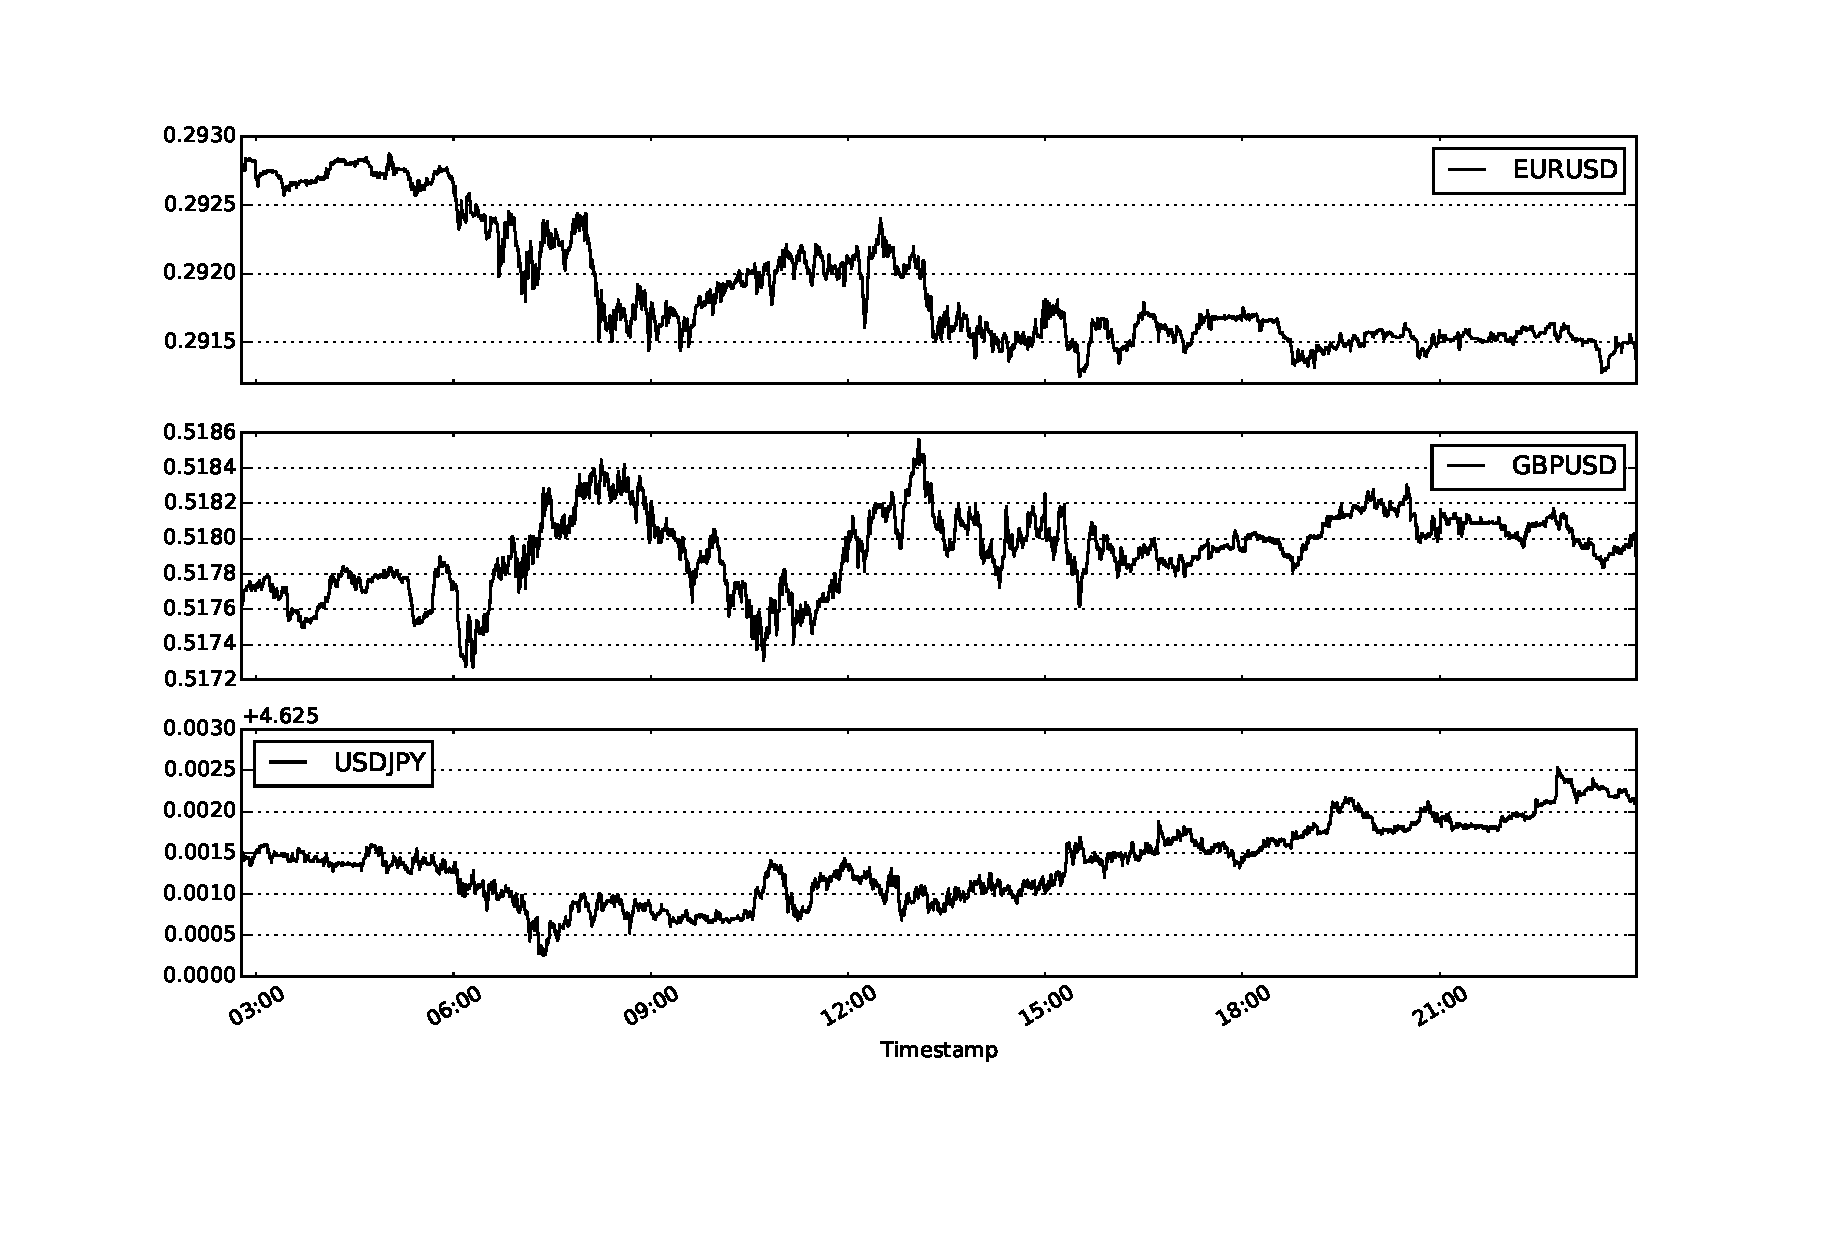
\includegraphics[scale=0.34]{forexdata}
  \caption{10 seconds frequency forex data for EURUSD, GBPUSD and USDJPY}
  \label{fig:forexdata}
\end{figure}

\begin{figure}[!ht]
  \vspace*{-1cm}
  \hspace*{-0.3in}
  \centering
  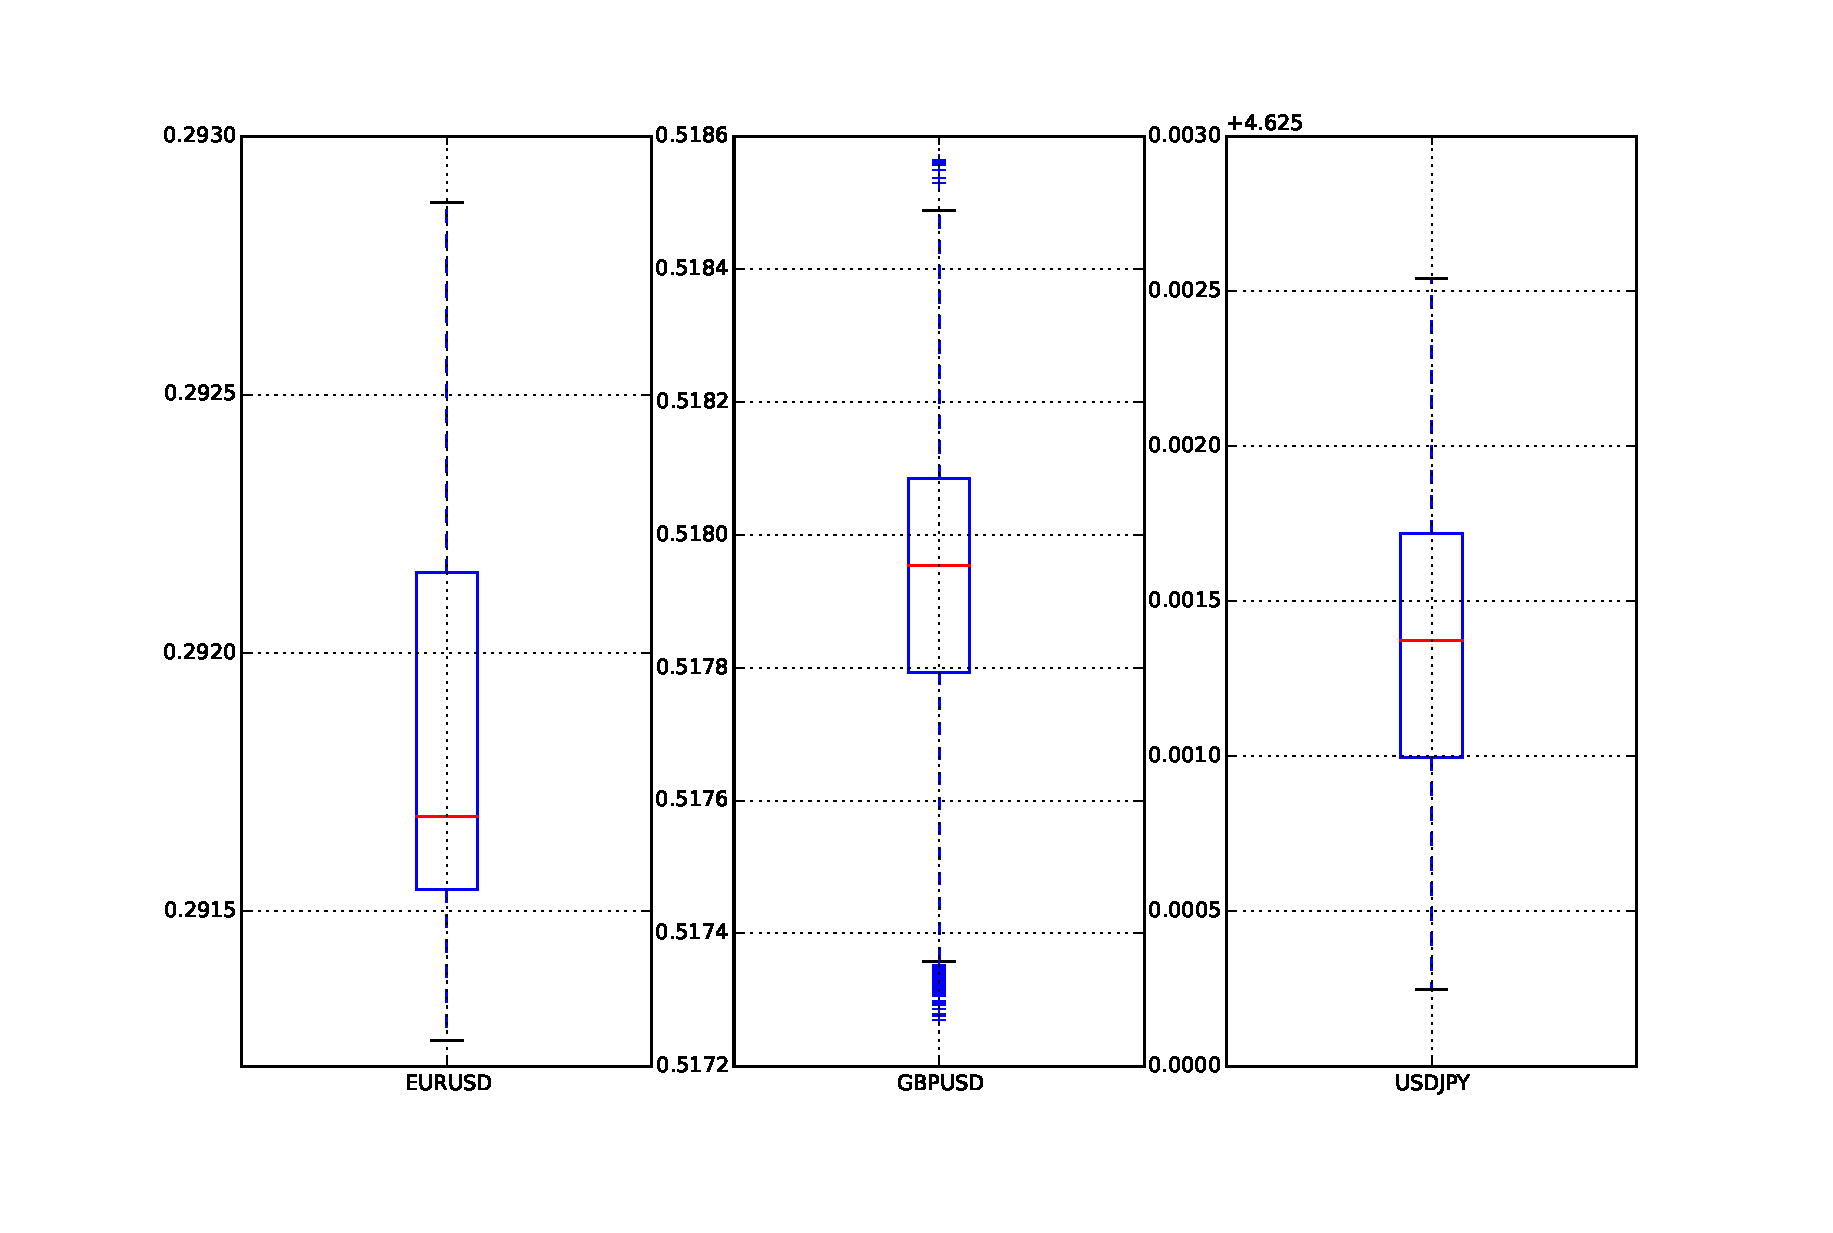
\includegraphics[scale=0.3]{distdata}
  \caption{Distribution of EURUSD, GBPUSD and USDJPY data}
  \label{fig:distdata}
\end{figure}

\subsection{Unit root tests} \label{sec:unitroot}
Before running the tests, we firstly checked whether the time series were
I(1) using the Augmented Dickey Fuller (ADF) \cite{dickey1979,dickey1981} test at 95\% significance level.
Table~\ref{tab:adf} shows that all currency rates cannot reject the unit root
test but they rejected it with their first differences. This means that all of
them are I(1) time series and we are allowed to use VECM and therefore OVECM.

\begin{table}[h!]
\label{tab:adf}
\begin{center}
\begin{tabular}{|l|c|c|c|c|c|}
\hline
& \textbf{Statistic} & \textbf{Critical value} & \textbf{Result}\\
\hline
EURUSD          &  -0.05398   & -1.94101 & True       \\
$\Delta$ EURUSD & -89.12344   & -1.94101 & False       \\
GBPUSD          &  -0.88208   & -1.94101 & True          \\
$\Delta$ GBPUSD & -82.56501   & -1.94101 & False       \\
CHFUSD          & -0.49941    & -1.94101 & True         \\
$\Delta$ CHFUSD & -74.21940   & -1.94101 & False       \\
\hline
\end{tabular}
\end{center}
\caption{Unit roots tests for EURUSD, GBPUSD and USDCHF at 10-seconds
frequency.}
\end{table}

\section{Experiments}

Competitive analysis were done considering the optimal offline algorithm (OOVECM). Cumulative loss is shown for different settings of OVECM. Figure \ref{fig:RRcomparison}  shows a comparison between OVECM using RR with different values for $\lambda$. It should be notice that RR with $\lambda = 0$ setting is equivalent to OLS. Experiments show that it is possible to reduce cumulative loss using some $\lambda \neq 0$.

\begin{figure}[!ht]
  %\vspace{-0.8cm}
  \centering
  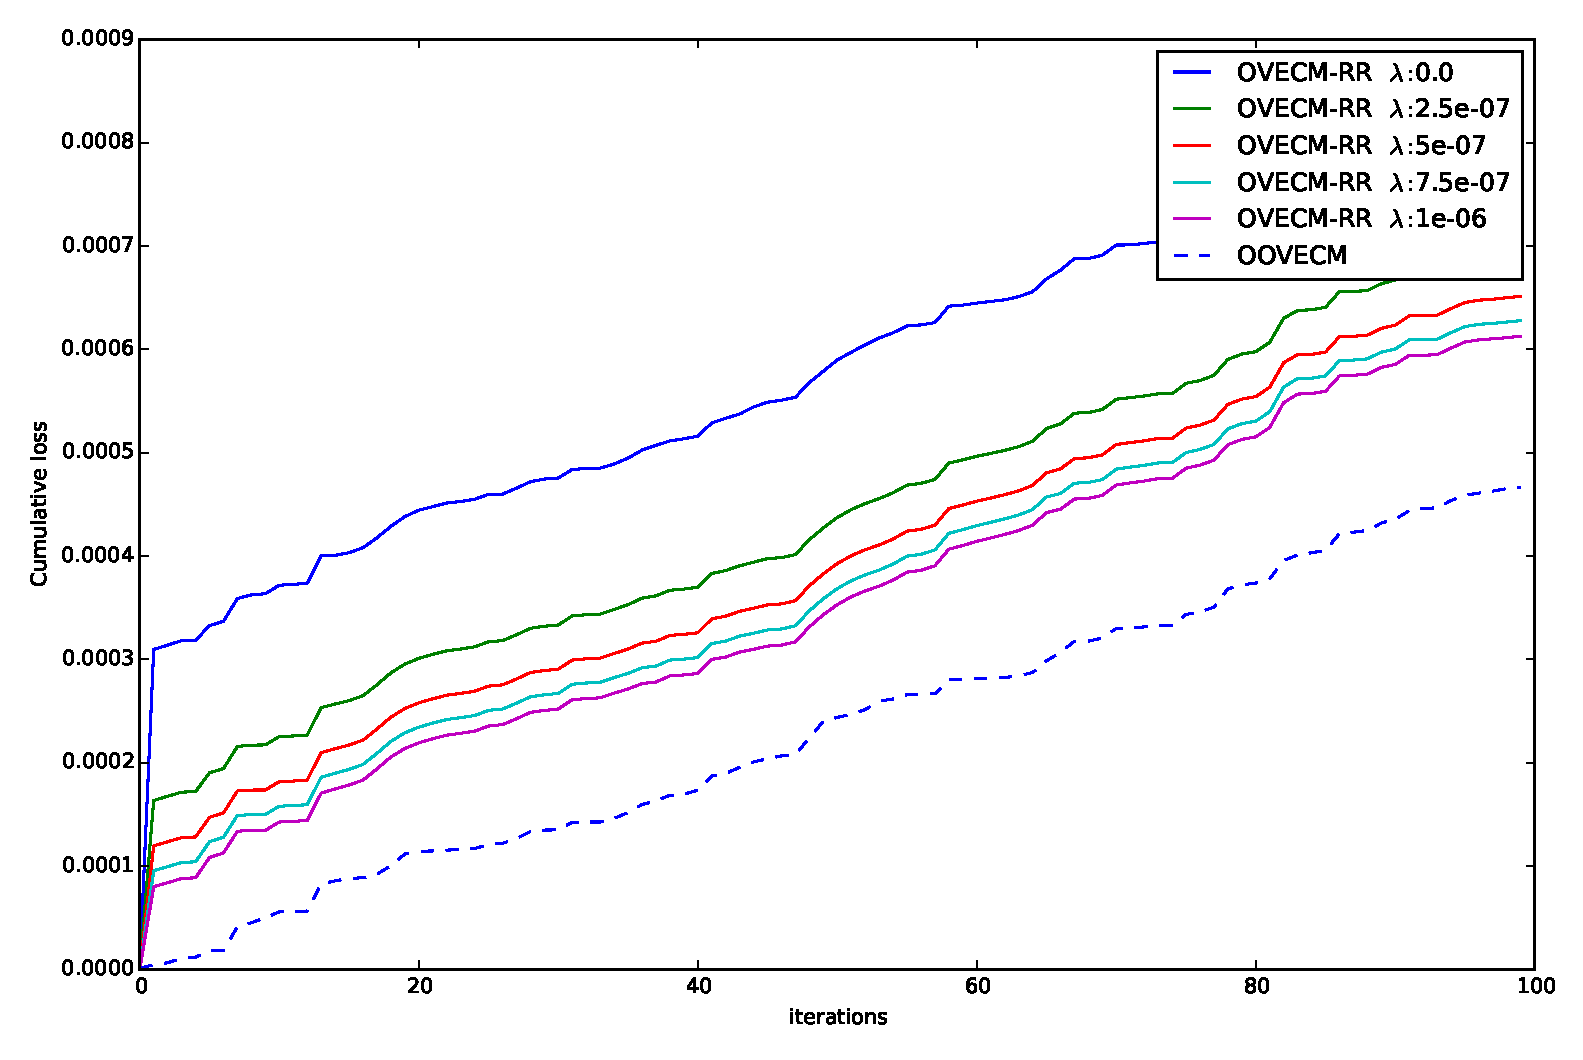
\includegraphics[width=0.5\textwidth]{RRcomparison}
  \caption{Cumulative loss RR VECM against its optimal algorithm using different $\lambda$ values}
  \label{fig:RRcomparison}
\end{figure}

Same experiments were done using the AAR setting for different values for $\lambda$. The effectiveness of the regularization parameter is so clear than RR. However, AAR seems to be a good predictor compared with OOVECM. Results are shown in figure \ref{fig:AARcomparison}.

\begin{figure}[!ht]
  %\vspace{-0.8cm}
  \centering
  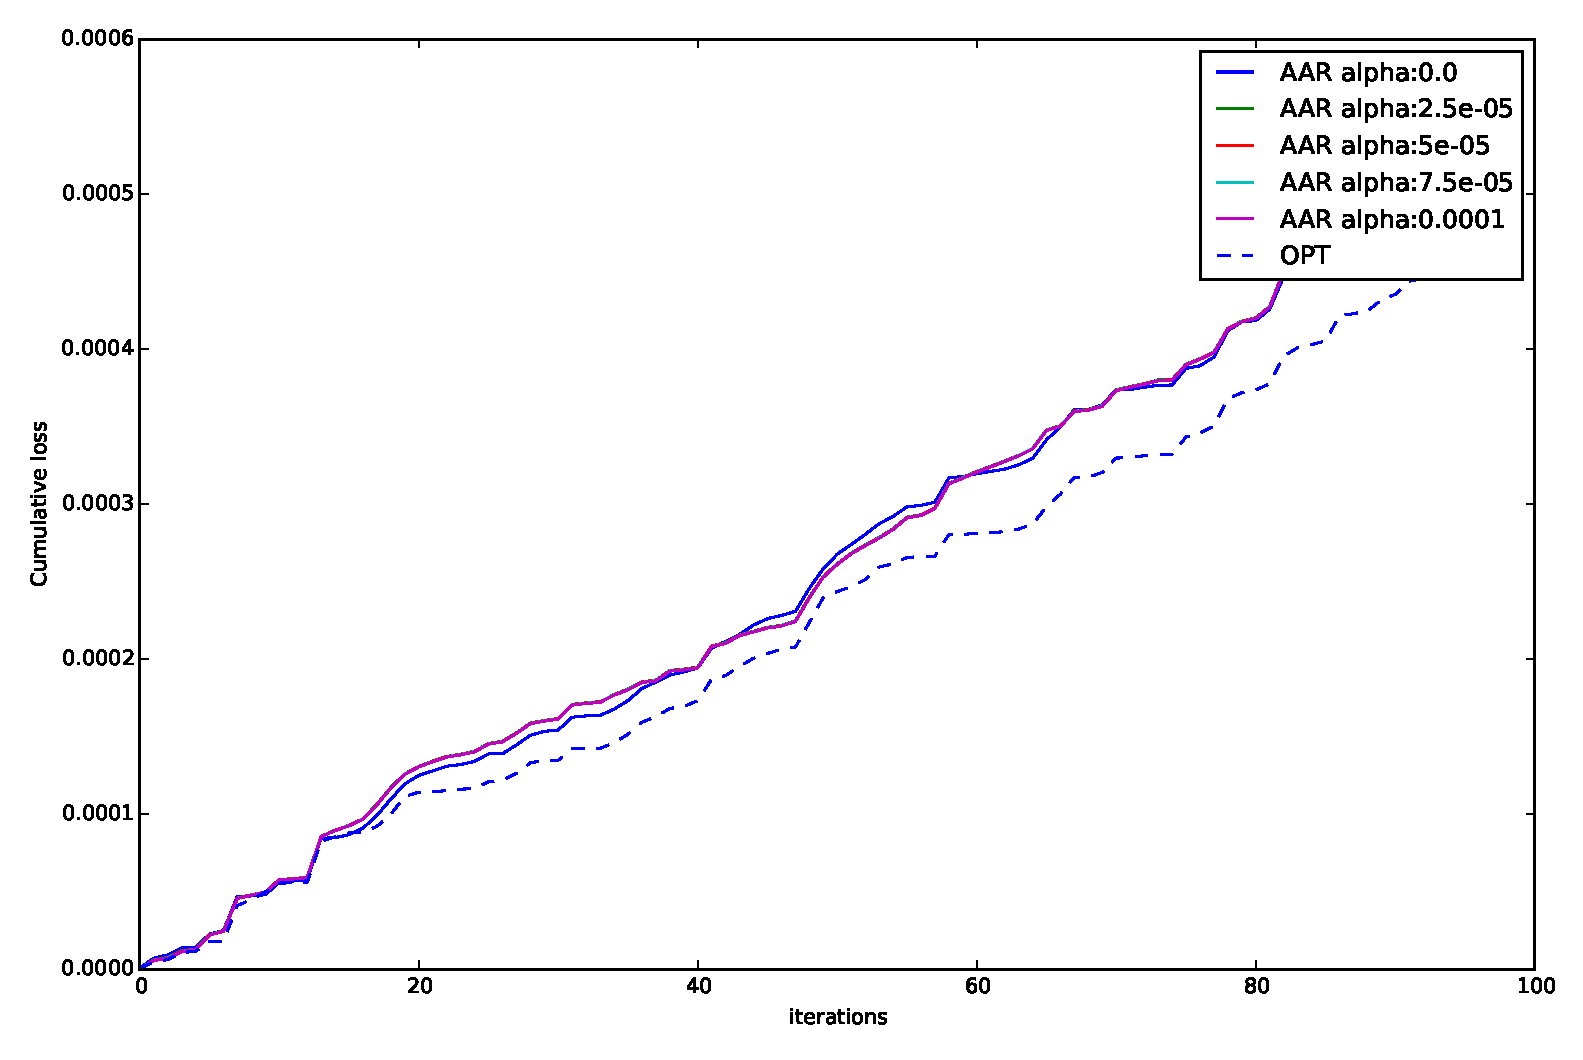
\includegraphics[width=0.5\textwidth]{AARcomparison}
  \caption{Cumulative loss AAR VECM against its optimal algorithm using different $\lambda$ values}
  \label{fig:AARcomparison}
\end{figure}

Finally, the three settings are compared with OOVECM. We can see that RR and AAR approaches are better than traditional OLS and also AAR seems to perform better than RR.

\begin{figure}[!ht]
  %\vspace{-0.8cm}
  \centering
  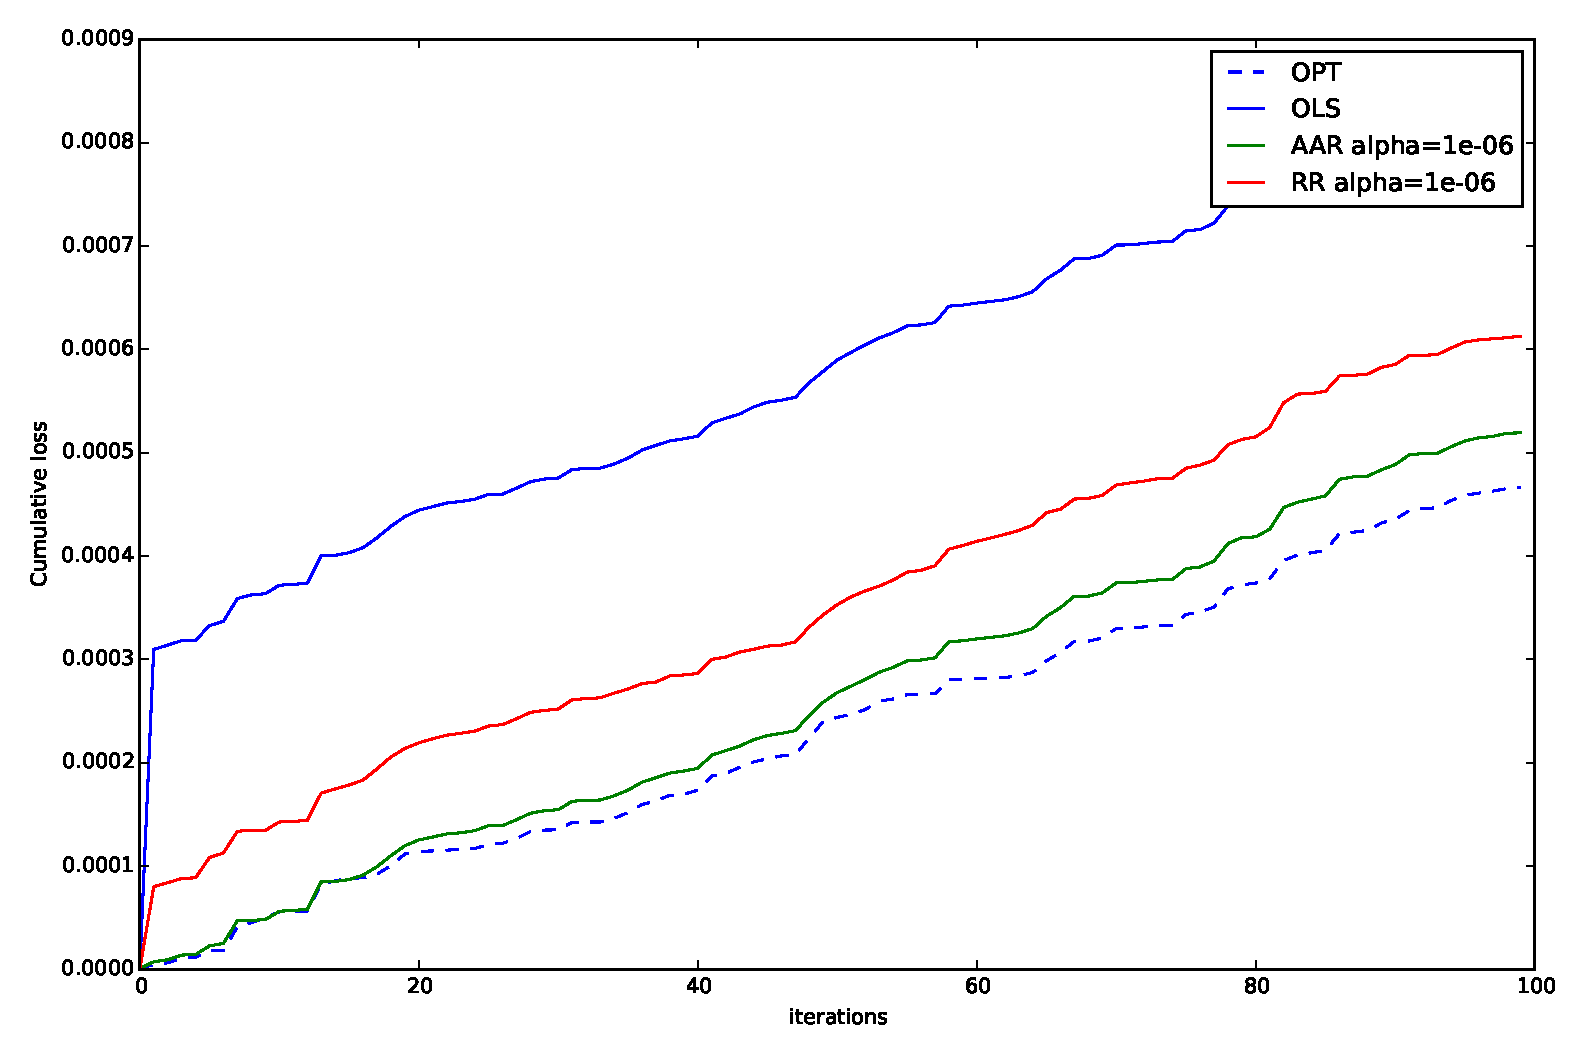
\includegraphics[width=0.5\textwidth]{onlinecomparison}
  \caption{Cumulative loss of AAR, RR and OLS solutions for VECM against its optimal algorithm}
  \label{fig:onlinecomparison}
\end{figure}


\section{Conclusions}
\label{sec:conclusions}

A new online version of the VECM has been proposed in order to use it with high frequency time series such as foreign exchange market rates. VECM takes advantage of the cointegration evidence between rates related to the USD currency. In order to get an online version we used the online versions of RR and AAR which are commonly used with problems with sequential access to the data. RR and AAR are used instead of the traditional OLS approach which has several known problems. A competitive analysis was done and experiments have shown that a regularised version OVECM could lead to improve cumulative losses compared with its optimal offline algorithm. Moreover, we showed that AAR could be a better option to improve performance independently of  how we choose $\lambda$ parameter. 

\bibliographystyle{plain}       % APS-like style for physics

\bibliography{reference}   % name your BibTeX data base

\end{document}
% end of file template.tex

